\documentclass{article}
\usepackage{amsmath}
\usepackage{mathptmx}
\usepackage{listofitems} % for \readlist to create arrays
\usepackage{tikz}
\usepackage{pgfplots}
\usepgfplotslibrary{colormaps}
\usepgfplotslibrary{patchplots}
\usepgfplotslibrary{polar}
\usepgfplotslibrary{fillbetween}
\usepackage{tkz-fct}
\usetikzlibrary{angles, quotes}
\usetikzlibrary{arrows.meta, arrows}
\usetikzlibrary{external}
\tikzexternalize[prefix={external/}]

\definecolor{myblue}{rgb}{0.067,0.529,0.871}
\definecolor{mypurple}{rgb}{0.859,0.071,0.525}
\definecolor{myred}{rgb}{1.0, 0.13, 0.32}
\definecolor{mygreen}{rgb}{0.01, 0.75, 0.24}
\definecolor{myblack}{gray}{0.5}
\definecolor{mygray}{gray}{0.7}

\pgfplotsset{
    compat=newest,
    colormap={bluemap}{color=(myblue) color=(myblue!25) color=(myblue!50)},
    colormap={redmap}{color=(myred) color=(myred!25) color=(myred!50)}
}

\tikzset{
    export as png/.style={
        external/system call/.add={}{
            && convert -density #1 -transparent white "\image.pdf" "\image.png"
        },
    },
    export as png/.default={200},
}

\DeclareSymbolFont{symbolsb}{OMS}{cmsy}{m}{n}
\SetSymbolFont{symbolsb}{bold}{OMS}{cmsy}{b}{n}
\DeclareSymbolFontAlphabet{\mathcal}{symbolsb}
\definecolor{myblue}{rgb}{0.067,0.529,0.871}
\definecolor{mypurple}{rgb}{0.859,0.071,0.525}
\definecolor{myred}{rgb}{1.0, 0.13, 0.32}
\definecolor{mygreen}{rgb}{0.01, 0.75, 0.24}
\definecolor{myblack}{gray}{0.5}
\definecolor{mygray}{gray}{0.7}

\def\req{\protect\rotatebox{90}{$\scriptstyle=$}}

\begin{document}

\tikzset{export as png}

\tikzsetnextfilename{red-neuronas}
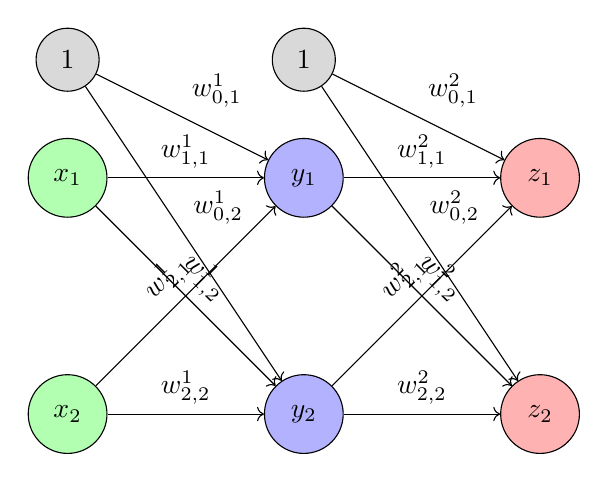
\begin{tikzpicture}
    % Define styles for layers and biases
    \tikzstyle{neuron}=[circle, draw, minimum size=1cm]
    \tikzstyle{input neuron}=[neuron, fill=green!30]
    \tikzstyle{hidden neuron}=[neuron, fill=blue!30]
    \tikzstyle{output neuron}=[neuron, fill=red!30]
    \tikzstyle{bias neuron}=[neuron, fill=gray!30, minimum size=0.8cm]
    
    % Input layer
    \node[input neuron] (I-1) at (0,1.5) {$x_1$};
    \node[input neuron] (I-2) at (0,-1.5) {$x_2$};
    \node[bias neuron] (B-I) at (0, 3) {1};

    % Hidden layer
    \node[hidden neuron] (H-1) at (3,1.5) {$y_1$};
    \node[hidden neuron] (H-2) at (3,-1.5) {$y_2$};
    \node[bias neuron] (B-H) at (3, 3) {1};

    % Output layer
    \node[output neuron] (O-1) at (6,1.5) {$z_1$};
    \node[output neuron] (O-2) at (6,-1.5) {$z_2$};

    % Connections: Input to Hidden layer with weights
    \foreach \i/\j in {1/1, 1/2, 2/1, 2/2} {
        \draw[->] (I-\i) -- (H-\j) node[midway, above, sloped] { $w^1_{\i,\j}$ };
    }
    \foreach \j in {1,2} {
        \draw[->] (B-I) -- (H-\j) node[midway, above right] {$w^1_{0,\j}$};
    }

    % Connections: Hidden to Output layer with weights
    \foreach \i/\j in {1/1, 1/2, 2/1, 2/2} {
        \draw[->] (H-\i) -- (O-\j) node[midway, above, sloped] { $w^2_{\i,\j}$ };
    }
    \foreach \j in {1,2} {
        \draw[->] (B-H) -- (O-\j) node[midway, above right] {$w^2_{0,\j}$};
    }

\end{tikzpicture}
\end{document}


